% Copyright 2025  Ed Bueler

\documentclass[10pt,hyperref]{beamer}

\mode<presentation>
{
  \usetheme{Madrid}

  \usecolortheme{beaver}

  \setbeamercovered{transparent}
  
  \setbeamerfont{frametitle}{size=\large}
}

\setbeamercolor*{block title}{bg=red!10}
\setbeamercolor*{block body}{bg=red!5}

\usepackage[english]{babel}
\usepackage[latin1]{inputenc}
\usepackage{times}
\usepackage[T1]{fontenc}
% Or whatever. Note that the encoding and the font should match. If T1
% does not look nice, try deleting the line with the fontenc.

\usepackage{empheq}
\usepackage{animate}
\usepackage{bm,xspace,verbatim,fancyvrb}
\usepackage{hyperref}

% If you wish to uncover everything in a step-wise fashion, uncomment
% the following command: 
%\beamerdefaultoverlayspecification{<+->}

\newcommand{\bb}{\mathbf{b}}
\newcommand{\bc}{\mathbf{c}}
\newcommand{\bbf}{\mathbf{f}}
\newcommand{\bg}{\mathbf{g}}
\newcommand{\br}{\mathbf{r}}
\newcommand{\bx}{\mathbf{x}}
\newcommand{\by}{\mathbf{y}}
\newcommand{\bv}{\mathbf{v}}
\newcommand{\bu}{\mathbf{u}}
\newcommand{\bw}{\mathbf{w}}

\newcommand{\bzero}{\bm{0}}

\newcommand{\grad}{\nabla}
\newcommand{\Grad}{\grad}
\newcommand{\Div}{\nabla\cdot}
\newcommand{\Curl}{\nabla\times}

\newcommand{\CC}{\mathbb{C}}
\newcommand{\RR}{\mathbb{R}}

\newcommand{\ddt}[1]{\ensuremath{\frac{\partial #1}{\partial t}}}
\newcommand{\ddx}[1]{\ensuremath{\frac{\partial #1}{\partial x}}}
\newcommand{\Matlab}{\textsc{Matlab}\xspace}
\newcommand{\Octave}{\textsc{Octave}\xspace}
\newcommand{\eps}{\epsilon}

\renewcommand{\Re}{\text{Re}}
\newcommand{\buold}{\bu^{\text{old}}}

\newcommand{\mfile}[1]{
\VerbatimInput[frame=single,label=\fbox{\scriptsize \textsl{\,#1\,}},fontfamily=courier,fontsize=\scriptsize]{#1}
}

\DefineVerbatimEnvironment{mVerb}{Verbatim}{numbersep=2mm,framerule=0.1mm,framesep=2mm,xleftmargin=4mm,fontsize=\small}


\AtBeginSection[]
{
  \begin{frame}<beamer>
    \frametitle{Outline}
    \tableofcontents[currentsection,hideallsubsections]
  \end{frame}
}

\title{Navier-Stokes solved with finite elements}

\subtitle{in Firedrake}

\author{Ed Bueler}

\institute{MATH 692 Fluids \& Solids Seminar}

\date{Spring 2025}


\begin{document}
\beamertemplatenavigationsymbolsempty

\begin{frame}
  \maketitle
\end{frame}


\begin{frame}{assumptions}

\begin{itemize}
\item all examples here are for 2D domains $\Omega \subset \RR^2$
\item notation: \, $\bu(t,x,y)$ is velocity and $p(t,x,y)$ is pressure
\item density $\rho>0$ is constant
    \begin{itemize}
    \item[$\circ$] fluid is incompressible
    \end{itemize}
\item dynamic viscosity $\mu>0$ is constant
    \begin{itemize}
    \item[$\circ$] constitutive relation: \, $\sigma = -p I + 2 \mu D\bu$
    \end{itemize}
\item body force set to zero: \, $\bbf = \bzero$

\bigskip
\item units: $[\bu]=\text{m}\,\text{s}^{-1}$, $[p]=\text{N}\,\text{m}^{-2}\,\text{s}^{-1}$, $[\rho]=\text{kg}\,\text{m}^{-3}$, $[\mu]=\text{kg}\,\text{m}^{-1}\,\text{s}^{-1}$
\end{itemize}
\end{frame}


\begin{frame}{the Navier-Stokes model}

\begin{itemize}
\item the time-dependent, incompressible, constant-viscosity Navier-Stokes equations are:
\begin{align*}
\rho\left(\bu_t + \bu \cdot \grad \bu\right) &= \mu \grad^2 \bu - \grad p & &\text{conservation of momentum} \\
\Div \bu &= 0 & &\text{incompressibility (c.~of mass)}
\end{align*}
\end{itemize}
\end{frame}


\begin{frame}{potential flow past a cylinder}

\begin{itemize}
\item recall from 2 weeks ago that Nick provided formula for the potential flow past a cylinder
\item in a \alert{potential flow} the vorticity is zero: \, $\bm{\omega}=\Curl\bu=\bzero$
\item incompressible potential flows satisfy:
\begin{align*}
\Curl \bu &= 0 & &\text{conservation of momentum} \\
\Div \bu &= 0 & &\text{incompressibility (c.~of mass)}
\end{align*}
\item zero curl ($\Curl\bu=0$) so there exists a potential $\bu = \grad \phi$
\item \dots and by incompressibility $\phi$ is harmonic: \, $\grad^2 \phi = 0$
\item assume far field velocity $\bu=(U_0,0)$
\item assume non-penetration and free slip on circle $r=a$
\item get by separation of variables:
	$$\phi(r,\theta) = U_0 \left(r + \frac{a^2}{r}\right) \cos(\theta) \hspace{2.3in}$$
\end{itemize}
\end{frame}


\begin{frame}{potential flow past a cylinder}

\begin{itemize}
\item potential:
	$$\phi(r,\theta) = U_0 \left(r + \frac{a^2}{r}\right) \cos\theta \hspace{2.3in}$$
\item velocity $\bu = \grad \phi$:
{\scriptsize
    $$\hspace{-4mm} \bu(r,\theta) = U_0 \left(1 - \frac{a^2}{r^2}\right) \cos\theta \,\hat \br - U_0 \left(1 + \frac{a^2}{r^2}\right) \sin\theta \,\hat \theta \hspace{3in}$$
}
\item \emph{however}, the boundary condition

along the cylinder, non-penetration

and free slip, is not realistic for

a viscous fluid
\item in fact there is substantial

vorticity along the cylinder
\item and flow separation \dots
\end{itemize}

\vspace{-50mm}
\hfill 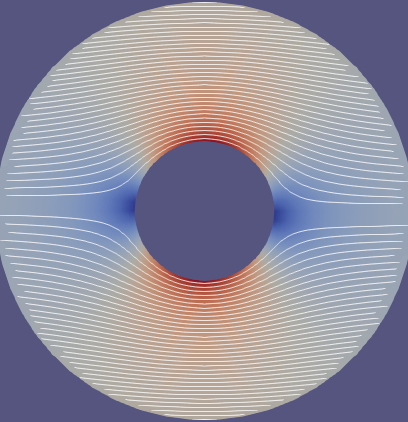
\includegraphics[width=0.45\textwidth]{figs/flowcyl.png}
\end{frame}


\begin{frame}{plan for today}

\begin{itemize}
\item use Firedrake to solve Navier-Stokes (NS) in two situations:
    \begin{enumerate}
    \item lid-driven cavity on a square \hfill \alert{$\leftarrow$ \emph{DEMO NOW!}}
    \item flow around a cylinder on a custom mesh
    \end{enumerate}

\bigskip
\item TO DO today:
    \begin{itemize}
    \item[$\circ$] the Reynolds scaling argument, to reduce \# of parameters
    \item[$\circ$] implicit discretization of Navier-Stokes (in time)
    \item[$\circ$] weak form
    \item[$\circ$] choice of finite element function spaces
    \item[$\circ$] practical Firedrake coding
    \item[$\circ$] visualization with Paraview
    \item[$\circ$] meshing with Gmsh
    \end{itemize}
\end{itemize}
\end{frame}


\begin{frame}{Reynolds number}

\begin{itemize}
\item recall NS equations:
\begin{align*}
\rho\left(\bu_t + \bu \cdot \grad \bu\right) &= \mu \grad^2 \bu - \grad p, \qquad 
\Div \bu = 0
\end{align*}
\item a particular simulation sets several scales:
    \begin{itemize}
    \item[] $\rho$ density
    \item[] $\mu$ dynamic viscosity
    \item[] $L$ (how long and wide is the domain?)
    \item[] $V$ (how fast is the fluid, e.g.~at boundaries?)
    \end{itemize}
\item one can change variables in the NS model using these substitutions:
    $$\bu = V \tilde \bu, \qquad p = \rho V^2 \tilde p, \qquad \grad = \frac{1}{L} \tilde \grad, \qquad \frac{\partial}{\partial t} = \frac{V}{L} \frac{\partial}{\partial \tilde t}$$

    \begin{itemize}
    \item[$\circ$] the new variables have tildes: \, $\bu,p,x,t \to \tilde \bu,\tilde p,\tilde x,\tilde t$
    \item[$\circ$] the new variables are dimensionless
    \end{itemize}
\end{itemize}
\end{frame}


\begin{frame}{Reynolds number}

\begin{itemize}
\item one rewrites the NS equations using the tilde variables \dots
\item drop the tildes:
\begin{align*}
\bu_t + \bu \cdot \grad \bu &= \frac{\mu}{\rho V L} \grad^2 \bu - \grad p, \qquad 
\Div \bu = 0
\end{align*}
\item note coefficient is dimensionless:
	$$\frac{[\mu]}{[\rho] [V] [L]} = \frac{(\text{kg}\,\text{m}^{-1}\,\text{s}^{-1})}{(\text{kg}\,\text{m}^{-3}) (\text{m}\,\text{s}^{-1}) (\text{m})} = 1$$
\end{itemize}
\begin{definition} the \emph{Reynold's number} is the dimensionless ratio
	$$\Re = \frac{\rho V L}{\mu}$$
\end{definition}
\end{frame}


\begin{frame}{Reynolds number}

\begin{itemize}
\item dimensionless NS equations used from now on ($\Re = \rho V L/\mu > 0$):
\begin{align*}
\bu_t + \bu \cdot \grad \bu &= \frac{1}{\Re} \grad^2 \bu - \grad p \\
\Div \bu &= 0
\end{align*}
\item if $\Re$ is small then viscosity is dominant
\item if $\Re$ is large then inertia is dominant
\end{itemize}
\end{frame}


\begin{frame}{implicit time steps}

\begin{itemize}
\item discretization in time typically uses finite differences
\item \emph{key idea}: there is no time derivative in the incompressiblity equation!
    \begin{itemize}
    \item[$\circ$] thus NS equations are really a ``differential-algebraic'' system in time, and infinitely stiff, thus implicitness is a good idea
    \end{itemize}
\item I will use $O(\Delta t)$ backward (implicit) Euler method, highly stable:
	$$\bu_t \approx \frac{\bu^{n} - \bu^{n-1}}{\Delta t}$$
\item suppose $\bu^{n-1}$ is known from previous time step, or initial condition
\item unknowns are $\bu^n$ and $p^n$:
\begin{align*}
\frac{\bu^{n} - \bu^{n-1}}{\Delta t} + \bu^n \cdot \grad \bu^n &= \frac{1}{\Re}\grad^2 \bu^n - \grad p^n \\
\Div \bu^n &= 0
\end{align*}

    \begin{itemize}
    \item[$\circ$] these equations are continuous in space
    \end{itemize}
\end{itemize}
\end{frame}


\begin{frame}{implicit time steps}

\begin{itemize}
\item cleaner notation $\bu=\bu^n$, $p=p^n$, $\buold = \bu^{n-1}$
\item also clear $\Delta t$ from denominator \dots get:

\begin{block}{implicit-step Navier-Stokes equations}
\begin{align*}
\bu - \buold + \Delta t \left(\bu \cdot \grad \bu - \frac{1}{\Re}\grad^2 \bu + \grad p\right) &= 0 \\
\Div \bu &= 0
\end{align*}
\end{block}

\item we will solve these equations for $\bu,p$ \alert{at every time step}, over the domain $\Omega$, using the boundary conditions, and using $\buold$ from the previous time step or the initial conditions
\end{itemize}
\end{frame}


\begin{frame}{weak form of NS equations}

\begin{itemize}
\item above equations are the ``strong form'', in which $\bu$ must have second derivatives and $p$ must have first derivatives
\item this is not necessary, and in a finite element (FE) method it is not desirable
\item technique: multiply first equation by test velocity $\bv$ and second equation by test pressure $q$, and then integrate
\begin{align*}
\int_\Omega (\bu - \buold)\cdot \bv + \Delta t \int_\Omega \left(\bu \cdot \grad \bu - \frac{1}{\Re}\grad^2 \bu + \grad p\right) \cdot \bv &= 0 \\
\int_\Omega (\Div \bu) q &= 0
\end{align*}
\end{itemize}
\end{frame}

\begin{frame}{}

\begin{itemize}
\item 
\end{itemize}
\end{frame}


\begin{frame}{}

\begin{itemize}
\item 
\end{itemize}
\end{frame}


\begin{frame}[fragile]{bar}

\begin{itemize}
\item foo
\begin{Verbatim}[fontsize=\small]
function [z, xk, k] = sdbt(f, x0, tol)

xk = x0(:);
maxiters = 10000;
for k = 1:maxiters
    [fk, dfk] = f(xk);           % objective and gradient
    if norm(dfk) < tol
        z = fk;
        break                    % success
    end
    pk = - dfk(:);               % steepest descent
    alpha = bt(xk, pk, dfk, f);  % back-tracking
    xk = xk + alpha * pk;
end
\end{Verbatim}
\end{itemize}
\end{frame}





\begin{frame}{summary}

\begin{itemize}
\item stuff
\item determining the step size $\alpha_k$, when actually taking the step, namely $x_{k+1}=x_k + \alpha_k p_k$, is nontrivial
    \begin{itemize}
    \item[$\circ$] line search (section 11.5) or trust region (11.6) is needed
    \item[$\circ$] for general functions, back-tracking is reasonable
    \item[$\circ$] for quadratic functions we can use the optimal step size
    \end{itemize}
\end{itemize}
\end{frame}




\end{document}

